\documentclass{article}%
\usepackage[T1]{fontenc}%
\usepackage[utf8]{inputenc}%
\usepackage{lmodern}%
\usepackage{textcomp}%
\usepackage{lastpage}%
\usepackage[head=40pt,margin=0.5in,bottom=0.6in]{geometry}%
\usepackage{graphicx}%
%
\title{\textbf{Rafaela Requesens: “Juan está incomunicado y aislado en una celda”}}%
\author{EL NACIONAL WEB}%
\date{11/10/2018}%
%
\begin{document}%
\normalsize%
\maketitle%
\textbf{URL: }%
http://www.el{-}nacional.com/noticias/politica/rafaela{-}requesens{-}juan{-}esta{-}incomunicado{-}aislado{-}una{-}celda\_255339\newline%
%
\textbf{Periodico: }%
EN, %
ID: %
255339, %
Seccion: %
Política\newline%
%
\textbf{Palabras Claves: }%
Política, Asamblea Nacional, Presos políticos, Sociedad\newline%
%
\textbf{Derecho: }%
1.2, %
Otros Derechos: %
1.10, %
Sub Derechos: %
1.2.2, 1.10.1.1\newline%
%
\textbf{EP: }%
NO\newline%
\newline%
%
\textbf{\textit{La hermana del preso político afirmó que "el régimen no tiene cómo demostrar que Juan es culpable"}}%
\newline%
\newline%
%
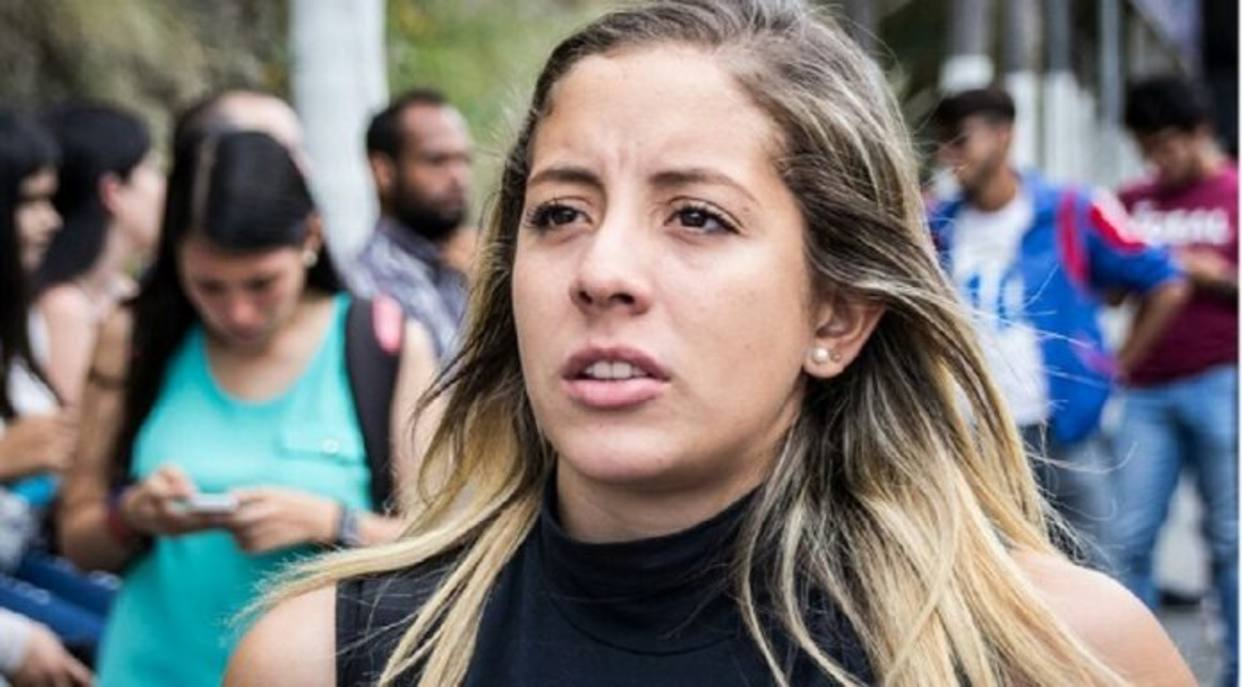
\includegraphics[width=300px]{193.jpg}%
\newline%
%
Rafaela Requesens, hermana del diputado a la Asamblea Nacional, Juan Requesens, indicó que su hermano se encuentra incomunicado y aislado en una celda del centro de reclusión de El Helicoide, reseñó~Diario ABC.%
\newline%
%
La hermana del diputado afirmó que hace dos días sus padres pudieron observarlo en la cárcel y hablar con él. "Juan les contó que estaba leyendo mucho sobre economía y analizando la crisis.~También pidió a los partidos que se unieran más allá de las diferencias personales para luchar contra el régimen", dijo.%
\newline%
%
Además agregó que temen diariamente por la vida de Requesens y que no han realizado la audiencia premilinar que debía efectuarse a los 45 días de la detención.%
\newline%
%
"El régimen no tiene cómo demostrar que Juan es culpable. En la vista preliminar~la juez no quiso agregar al expediente los vídeos~en el que mi hermano supuestamente se incrimina del atentado. Igual sabemos que van a manipular y sembrar información para imputarlo", aseguró.%
\newline%
%
Con información de~Diario ABC%
\newline%
%
\end{document}